\chapter{Overview of the LHCb upgrade}
\label{ref:lhcb-upgrade-overview}

% General changes
The run 2 of LHC has reached its conclusion at the end of 2018.
It has entered the second long shutdown (LS2) period since then.
During this period,
the upgrade on the LHC has enabled the accelerator to operate at
an unprecedented center of mass energy $\sqrt{s} = 13.6$~TeV with an
instantaneous luminosity of up to $2 \times 10^{33}$~cm$^{-2}$~s$^{-1}$ (a
five-fold increase compared to run 2's number)
\cite{CERN_news:2022,Piucci_2017}.
As of now\footnote{
    As a reminder, ``now'' refers to November 2022.
}, some of the LHCb subdetectors, for example the Upstream Tracker, are still
being upgraded.

% Motivate the LHCb upgrade
The upgraded LHC, however, poses an unique problem for the LHCb experiment:
the run 2 \pt-based hadronic trigger yields saturate at current luminosity which means
no increse in event yield as luminosity increase with currently hardware.
as shown in \cref{fig:l0-trigger-eff}.
to fix the problem, it is required to readout the full detector instead of triggering
on \pt only.
to do this, the full detector has to be read out at the LHC bunch crossing rate,
40~Mhz, far exceeding current capability of 1~MHz readout rate.

\begin{figure}[!htb]
    \centering
    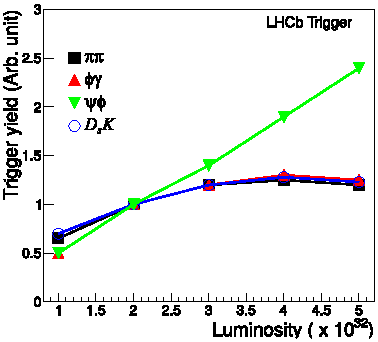
\includegraphics[width=0.5\textwidth]{./figs-lhcb-upgrade-overview/trigger_efficiency.pdf}
    \caption{
        L0 trigger yields for LHCb run 1 and 2.
        The hadronic triggers are already saturated at run 2 luminosity.
    }
    \label{fig:l0-trigger-eff}
\end{figure}

\begin{figure}[!htb]
    \centering
    \begin{subfigure}[t]{0.45\textwidth}
        \centering
        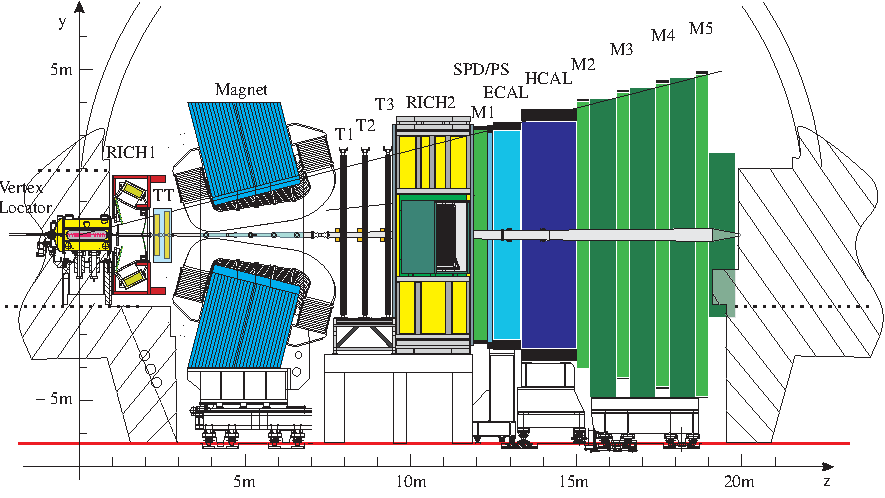
\includegraphics[width=\textwidth]{./figs-detector/lhcb_detector_view.pdf}
        \caption{The LHCb detector, run 1 and 2.}
    \end{subfigure}
    \hspace{12pt}
    %%%%
    \begin{subfigure}[t]{0.45\textwidth}
        \centering
        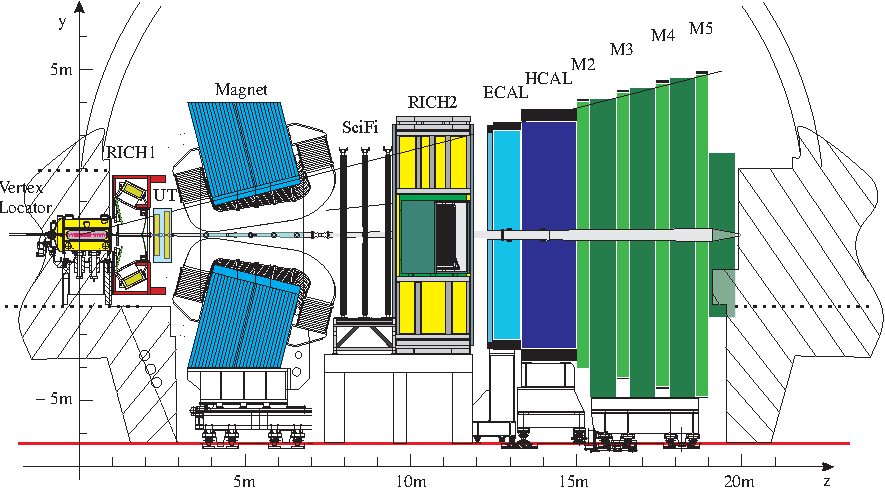
\includegraphics[width=\textwidth]{./figs-lhcb-upgrade-overview/lhcb_detector_view_run3.pdf}
        \caption{The upgraded LHCb detector in run 3.}
    \end{subfigure}

    \caption{
        The LHCb detector before (left) and after (right) LS2 upgrade.
    }
    \label{fig:lhcb-detector-comparison}
\end{figure}

The remaining chapter provides an overview of the LHCb detector upgrade in LS2.
\cref{ref:lhcb-upgrade-overview:readout} describes the upgrade of the detector
readout system across all subdetectors.
Some subdetectors are undergoing upgrade to improve its performance, notably
the tracking and the PID system;
these will be discussed in \cref{ref:lhcb-upgrade-overview:tracking} and
\cref{ref:lhcb-upgrade-overview:tracking}, respectively.
Finally,
\cref{ref:lhcb-upgrade-overview:hlt}
provides an comparison of the trigger schemes between run 2 and run 3 and
explains how the detector upgrade solves the trigger bottleneck.


\section{Detector readout}
\label{ref:lhcb-upgrade-overview:readout}


\section{Tracking system}
\label{ref:lhcb-upgrade-overview:tracking}

% Get a figure for old IT/OT combo vs. the new SciFi


\section{Particle identification system}
\label{ref:lhcb-upgrade-overview:tracking}


\section{High-level triggers in run 2 and run 3}
\label{ref:lhcb-upgrade-overview:hlt}
